\begin{figure}[t]\centering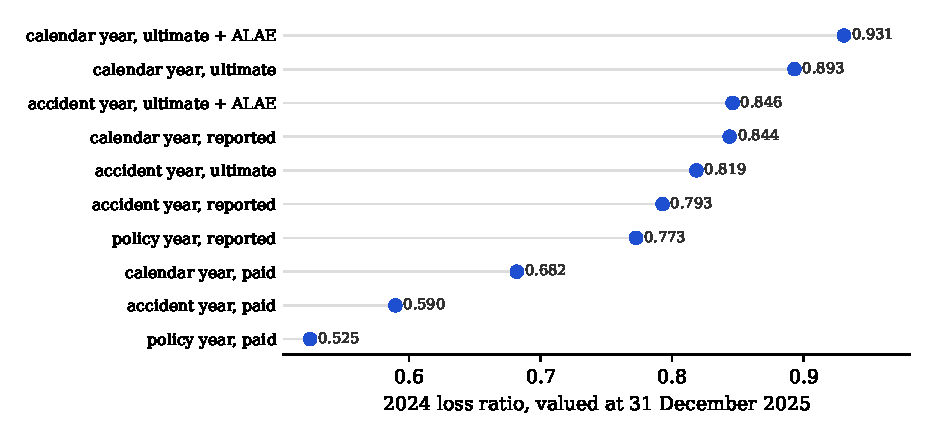
\includegraphics[width=\linewidth]{figures/answers.pdf}
\caption{Every defensible answer to ``what was the 2024 loss ratio?'' on the synthetic book, valued at 31
December 2025, as computed by the semantic layer. Ultimate figures include booked IBNR; the policy-year basis
has no booked IBNR, so no policy-year ultimate exists.}\label{fig:answers}\end{figure}

\begin{figure}[t]\centering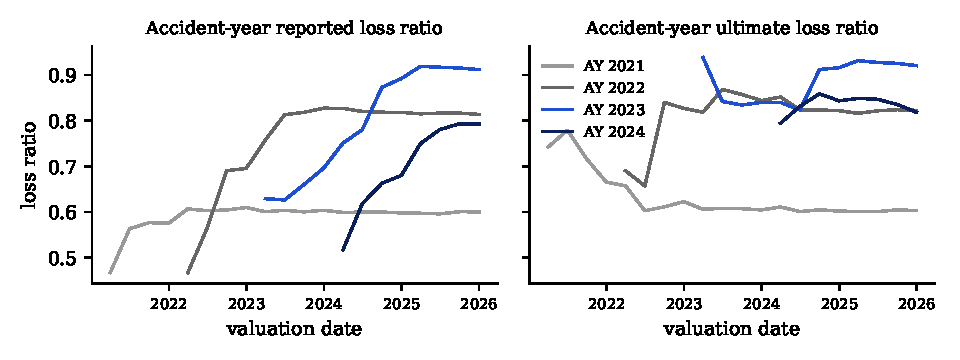
\includegraphics[width=\linewidth]{figures/development.pdf}
\caption{The same accident year read at successive quarter-end valuation dates. Reported loss ratios rise as
late claims are reported and reserves develop; adding booked IBNR anticipates much of that development.}
\label{fig:development}\end{figure}

\begin{table}[t]\centering\small
\caption{ISL-Bench results. Accuracy over all questions with a 95\% bootstrap interval over questions; accuracy on the answerable, unambiguous core; ambiguous questions answered with a defensible value (and, in brackets, how many answers named a basis or definition); unanswerable questions declined; wrong answers (in brackets, how many quoted the governed figure in their explanation); API cost.}\label{tab:main}
\resizebox{\linewidth}{!}{\begin{tabular}{llrrrrrr}\toprule
Model & Condition & All & Core & Ambiguous (disclosed) & Unanswerable & Wrong (quoted) & Cost \\ \midrule
Haiku 5.5 & raw & 77\% [66\%, 87\%] & 73\% & 7/7 (7) & 4/4 & 14 (7) & \$0.13 \\
Haiku 5.5 & docs & 98\% [95\%, 100\%] & 98\% & 7/7 (7) & 4/4 & 1 (1) & \$0.07 \\
Haiku 5.5 & semantic & 100\% [100\%, 100\%] & 100\% & 7/7 (7) & 4/4 & 0 (0) & \$0.02 \\
Sonnet 5.5 & raw & 84\% [74\%, 94\%] & 82\% & 7/7 (7) & 3/4 & 10 (3) & \$0.88 \\
Sonnet 5.5 & docs & 98\% [95\%, 100\%] & 100\% & 7/7 (7) & 3/4 & 1 (0) & \$0.58 \\
Sonnet 5.5 & semantic & 100\% [100\%, 100\%] & 100\% & 7/7 (7) & 4/4 & 0 (0) & \$0.39 \\
\bottomrule\end{tabular}}\end{table}

\begin{table}[t]\centering\small
\caption{Correct answers by question category (number of questions in brackets).}\label{tab:categories}
\resizebox{\linewidth}{!}{\begin{tabular}{lrrrrrr}\toprule
Category & Haiku raw & Haiku doc & Haiku sem & Sonnet raw & Sonnet doc & Sonnet sem \\ \midrule
Control (7) & 7/7 & 7/7 & 7/7 & 7/7 & 7/7 & 7/7 \\
Earning (6) & 5/6 & 5/6 & 6/6 & 6/6 & 6/6 & 6/6 \\
Time basis (8) & 3/8 & 8/8 & 8/8 & 5/8 & 8/8 & 8/8 \\
Valuation (5) & 2/5 & 5/5 & 5/5 & 2/5 & 5/5 & 5/5 \\
Loss definition (7) & 5/7 & 7/7 & 7/7 & 7/7 & 7/7 & 7/7 \\
Aggregation (7) & 4/7 & 7/7 & 7/7 & 4/7 & 7/7 & 7/7 \\
Snapshot (5) & 5/5 & 5/5 & 5/5 & 5/5 & 5/5 & 5/5 \\
Counting (2) & 2/2 & 2/2 & 2/2 & 2/2 & 2/2 & 2/2 \\
Retention (4) & 4/4 & 4/4 & 4/4 & 4/4 & 4/4 & 4/4 \\
Ambiguous (7) & 7/7 & 7/7 & 7/7 & 7/7 & 7/7 & 7/7 \\
Unanswerable (4) & 4/4 & 4/4 & 4/4 & 3/4 & 3/4 & 4/4 \\
\midrule Mean tool calls & 4.5 & 2.2 & 1.1 & 2.8 & 1.1 & 1.0 \\
\bottomrule\end{tabular}}\end{table}

\begin{table}[t]\centering\small
\caption{Every incorrect answer, classified from the model's own explanation. The first three classes are house conventions that cannot be discovered from raw tables.}\label{tab:errors}
\resizebox{\linewidth}{!}{\begin{tabular}{lrrrrrr}\toprule
Error class & Haiku raw & Haiku doc & Haiku sem & Sonnet raw & Sonnet doc & Sonnet sem \\ \midrule
ALAE included in losses & 9 & 0 & 0 & 7 & 0 & 0 \\
Recoveries not netted & 2 & 0 & 0 & 2 & 0 & 0 \\
Day-count convention & 2 & 1 & 0 & 0 & 0 & 0 \\
Wrong cohort definition & 1 & 0 & 0 & 0 & 0 & 0 \\
Answered a different question & 0 & 0 & 0 & 0 & 1 & 0 \\
Estimated instead of declining & 0 & 0 & 0 & 1 & 0 & 0 \\
\bottomrule\end{tabular}}\end{table}

% Hand-written narrative for Section 7. Every number is a macro from generated/numbers.tex
% or a cell in the generated tables, so it moves with the data.

\paragraph{One question, many answers.}
Figure~\ref{fig:answers} shows the problem the paper starts from: \HeadlineCount{} defensible values for the
2024 loss ratio, from \HeadlineMin{} (policy year, paid) to \HeadlineMax{} (calendar year, ultimate including
ALAE). None of them is an error. Figure~\ref{fig:development} shows why the valuation date has to be part of
the question. The reported loss ratio for accident years 2022--2024, read at their own year end and again at the horizon,
rises by 11 to 22 points as late claims arrive and reserves develop. Booked IBNR anticipates most of that
movement: the ultimate ratio moves by under three points for 2022 and 2024, but by eight points for 2023, the
year in which claims inflation outran the development pattern the chain ladder had learned.

\paragraph{Accuracy.}
Table~\ref{tab:main} reports accuracy against the governed definitions. With raw tables, Haiku~5.5 answers
\AccHaikuRaw{} of questions correctly and Sonnet~5.5 \AccSonnetRaw{}. With the glossary both reach
\AccHaikuDocs{}, and through the semantic layer both answer every question correctly. Every condition handled
the ambiguous questions with a defensible value and named its interpretation. Every condition except
Sonnet's two SQL conditions declined all four unanswerable questions (below).

\paragraph{What the raw-schema errors are.}
Table~\ref{tab:errors} classifies every wrong answer from the model's own explanation. The striking result is
how few of them are reasoning errors. No model confused calendar with accident year, used written for earned
premium, ignored a stated valuation date, averaged quarterly ratios, or summed a balance across periods. Those
are the misreadings the benchmark's traps were designed to catch, and none was triggered. \ConvErrRawHaiku{} of Haiku's
\WrongRawHaiku{} raw-schema errors, and \ConvErrRawSonnet{} of Sonnet's \WrongRawSonnet{}, are \emph{house
conventions} that no schema reveals. The three conventions are:
\begin{itemize}
\item whether ``reported'' or ``incurred'' losses include ALAE, which the models mostly included and the house
definition excludes;
\item whether paid losses are net of subrogation and salvage recoveries;
\item whether the valuation day itself is earned.
\end{itemize}
The models usually said which choice they made, and in \GoldMentionedRawHaiku{} (Haiku) and
\GoldMentionedRawSonnet{} (Sonnet) cases they quoted the governed figure as the alternative. Counting those
convention choices as correct, raw-schema accuracy would be \AdjRawHaiku{} for Haiku and \AdjRawSonnet{} for
Sonnet. On this benchmark, then, a current model with database access and no documentation gets the
\emph{reasoning} right and the \emph{conventions} wrong. The one genuine reasoning error is Haiku building a
policy-year cohort from each policy's first inception date rather than each term's.

\paragraph{Refusals.}
Sonnet with raw tables answered one unanswerable question, the booked policy-year ultimate loss ratio. It
allocated accident-year IBNR to policy years in proportion to incurred losses and said so. That is a reasonable
actuarial estimate, but not a booked figure, and the governed layer declines it. Sonnet with the glossary
answered ``loss ratio for windscreen claims'' with windscreen's contribution to the total loss ratio, and said
that too. Through the semantic layer, both models declined all four, and the refusal text was the compiler's
reason (premium is not split by peril; IBNR is booked by accident year and not allocated to channels).

\paragraph{Cost and effort.}
The semantic layer is also the cheapest condition (Table~\ref{tab:main}). Sonnet's whole run cost
\$0.39 through the semantic layer against \$0.88 with raw tables, and it needed far fewer tool calls
(Table~\ref{tab:categories}). Raw-schema runs spend most of their calls profiling tables and reconciling
movements before they compute anything.

\paragraph{What the benchmark found in the benchmark.}
Two findings were about our own artefacts, and we report them because they illustrate the paper's argument.
First, in the pilot both models' raw-SQL answers for earned exposure disagreed with our gold value by 3.5\%. The
models were right: the generator booked a full car-year of negative exposure on cancellation instead of the
unexpired fraction. We fixed the generator, added a regression test that reconciles earned exposure with
covered days, and re-ran the affected questions. Second, Sonnet with raw tables declined the 2025 expense ratio.
Its reason was that December's expenses are booked in January, so at 31 December 2025 the year is incomplete.
The semantic layer had happily divided eleven months of expenses by twelve months of premium. Valuation dates
make incompleteness \emph{visible} in the data, but our layer does not yet \emph{flag} it (Section~\ref{sec:discussion}).
We moved the two expense questions to 2024, and added to one ambiguous question (``incurred losses'') the
readings that include ALAE. All changes were made after the pilot and are marked in the questions file.

